\section{第一章\ 创世之光：你的第一个在线世界}
% 胡文举
在本书中，我们会用一款“玩法做减法、工程约束不打折”的在线对战游戏贯穿全篇：不去堆复杂系统，而是专盯在线服务绕不开的四件事：要快（低延迟的实时交互）、要一致（多人看到同一份世界状态）、要公平（由服务器做权威裁决）、还要能扛（流量一上来不崩、长期稳定在线）。实时多人游戏通常同时面临低延迟与高可用的硬要求，并且玩家规模会随时间与事件出现明显峰谷波动，因此非常适合作为理解云计算与分布式系统的一块“练兵场”。

因此，第一章不会急于进入代码细节，而是作为动工前的“总蓝图”，致力于帮助读者建立全局的系统认知。我们将首先梳理全书的架构演进框架，阐明从单机闭环到云原生集群的必然路径；随后，我们将提前展示贯穿后续章节的核心技术设定，即我们将搭建怎样的“兵工厂”来支撑这一庞大系统的运转。通过统一概念、划定边界与明确目标，我们希望让读者在真正敲下第一行代码之前，就能清晰地理解系统将在哪里承压、为何选择特定的技术路线，以及这些技术又是如何像流水线一样一步步组装起这个在线世界的。


% 需要改一下

\subsection{梦开始的地方：构建游戏设计蓝图}

% 首先要把全文的设定讲出来 -> 为什么要用在线游戏来学习云计算

\subsubsection{从网络游戏到在线系统工程}\label{subsubsec:从网络游戏到云计算项目} % 把网络游戏的设计过程 抽象成为工程问题 1.1.1

从表面看，一款网络游戏似乎只是一个“能联网一起玩”的应用：玩家登录账号，在地图中移动角色，与其他玩家交流或对战。但如果从系统工程的角度来看，它并不是一个简单的软件，而更像是一套围绕着“多人共享同一个世界”所构建的复杂系统。

可以想象这样一个场景：十几名玩家同时站在同一片游戏地图中。如果其中一名玩家释放了技能，其他玩家是否能在几毫秒内看到对应的效果？如果一名玩家突然掉线，重新连接后是否还能回到原来的位置？如果服务器出现故障，玩家辛苦积累的角色数据是否会全部丢失？这些问题并不属于游戏玩法本身，而是由底层系统来负责解决的工程问题。
正是因为需要应对这些问题，网络游戏在系统层面必须受到一系列工程约束的限制。例如：系统如何校验玩家身份并允许其接入？世界中发生的事件如何在多名玩家之间保持一致？在网络延迟和抖动不可避免的情况下，实时交互如何仍然保持“手感”可接受？关键数据又如何在断线、重启甚至硬件故障后被安全地恢复？这些约束共同决定了网络游戏系统的整体结构。

也正因如此，网络游戏成为理解现代在线服务架构的一个理想样本。它几乎涵盖了云计算和分布式系统中的所有典型问题：并发请求、状态同步、数据一致性、容错恢复以及资源调度等。对于传统的网络游戏而言，其整体架构通常可以抽象为如图 \ref{fig:chapter1-fig5} 所示的形式。

\begin{figure*}[htbp]
    \centering
    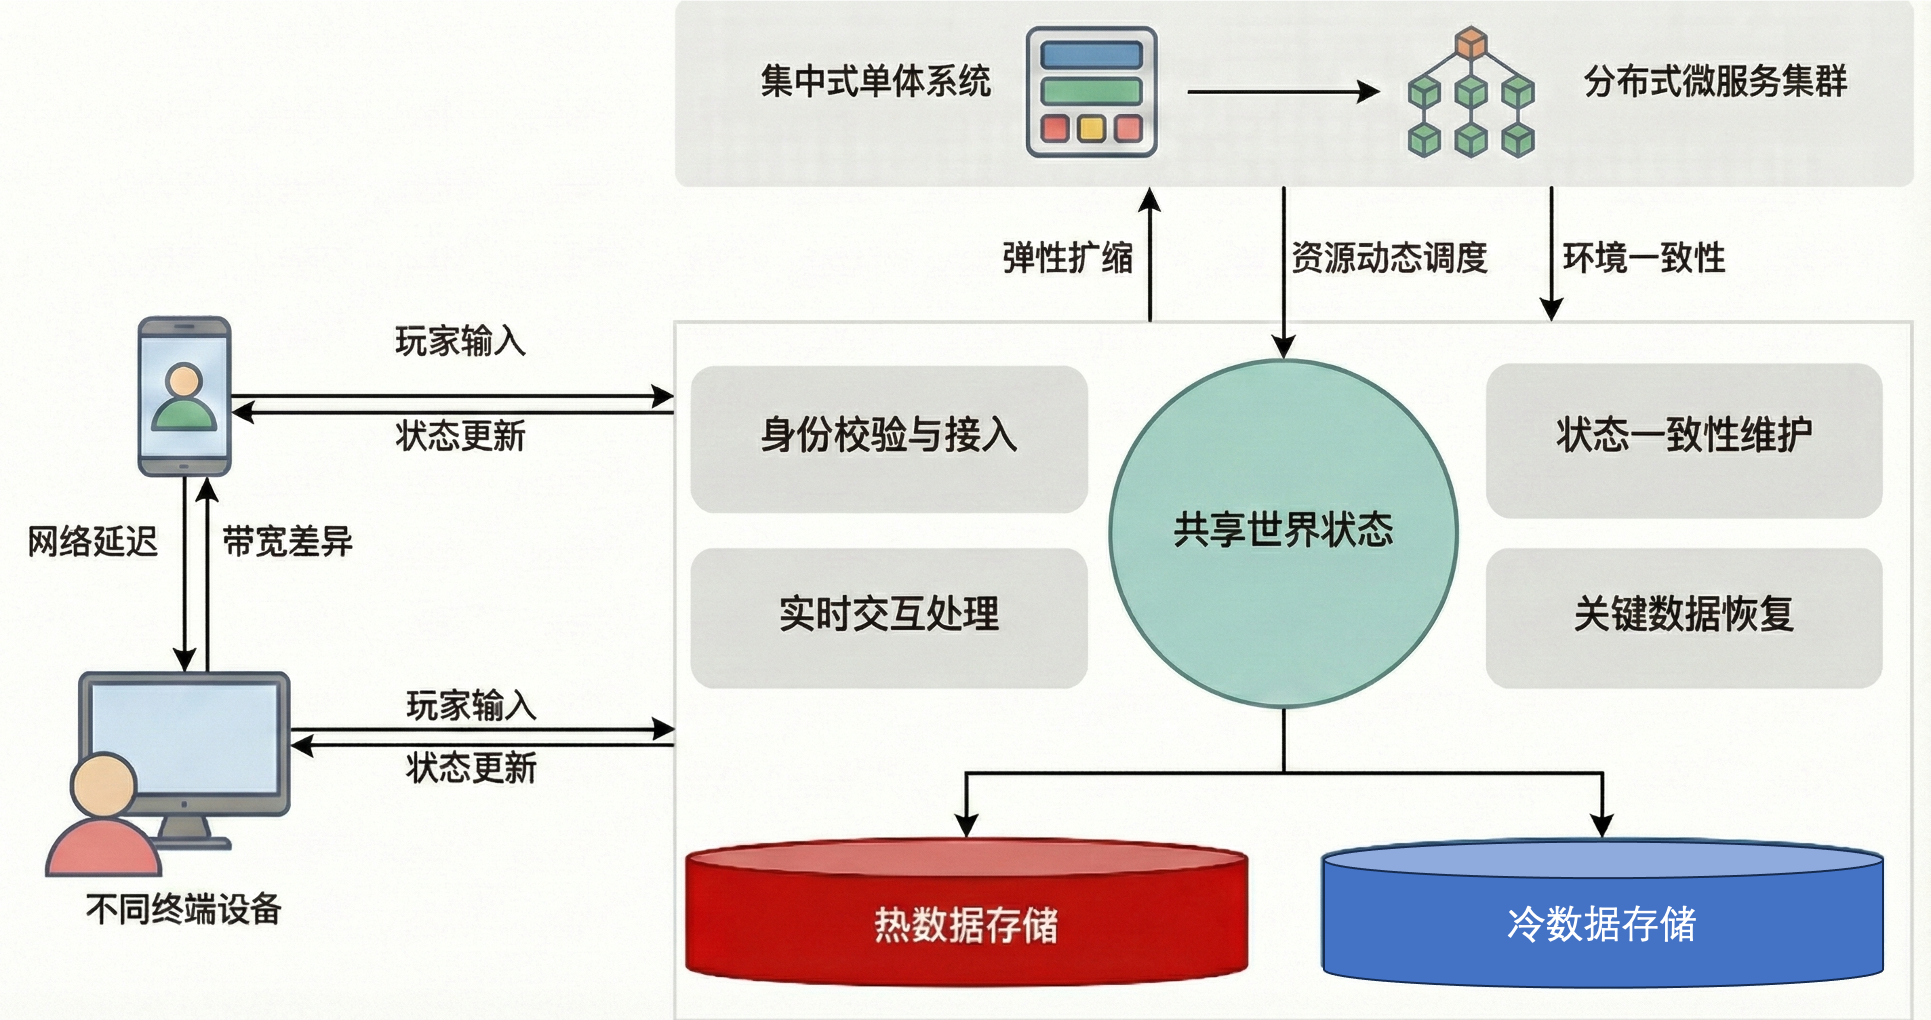
\includegraphics[width=1\linewidth,keepaspectratio]{figures/sec1/chapter1_structure2.png}
    \caption{游戏架构示意图}
    \label{fig:chapter1-fig5}
\end{figure*}

对于网络对战类游戏来说，真正的挑战并不仅仅是“让玩家连上服务器”，而是在多种现实条件的限制下，长期、稳定地运行一个多人在线系统。从更宏观的角度看，这类挑战并不只存在于游戏中，大多数大型网络应用——例如社交平台、电商系统或在线协作工具，同样会遇到类似的问题。因此，网络游戏可以被视为研究现代分布式系统的一种典型案例。

首先，任何云计算项目都必须解决一个最基本的问题：不同终端之间如何保持状态一致。每名玩家都运行在不同的设备上，网络延迟、带宽状况以及设备性能各不相同。如果完全依赖本地计算，很容易出现“我看到你已经倒下，但你自己却还在移动”的矛盾情况。为避免这种现象，系统通常需要引入服务器集中裁决、状态快照以及增量同步等机制，确保所有玩家对游戏世界的理解是统一且可信的。

其次，这类系统中的数据并非同等重要、同等紧急。以游戏为例，玩家的位置、速度和血量等信息需要被频繁更新，对延迟极为敏感；而账号信息、道具记录或任务进度则更新频率较低，但必须长期可靠保存。这种明显的“冷热数据”差异，决定了系统需要采用不同的存储方式来分别处理它们，这也是云计算项目中最基础的数据管理问题之一。

在项目早期，为了降低开发复杂度，系统往往采用集中式结构：所有功能运行在同一个服务进程中。此时系统逻辑清晰，部署简单，适合快速验证想法。但随着用户数量增加，同一时间需要处理的请求和状态更新急剧上升，顺序执行的处理方式会逐渐暴露出性能瓶颈。共享资源的竞争会导致锁等待、请求排队以及明显的响应延迟，单体系统的内部调度机制也难以支撑高并发需求。

当系统进一步扩展，功能模块增多、业务流程变复杂时，单台机器在计算能力、存储空间和网络带宽方面都不可避免地成为限制因素。不同模块对资源的需求差异明显，使集中式系统难以在各类需求之间取得平衡。同时，用户访问往往具有明显的地域分布和时间规律，系统必须依赖多台机器协同工作。这一阶段的核心问题，从单个节点内的多线程高并发转变为如何在多个节点之间划分任务、保持数据一致，并协调不同服务之间的依赖关系。

当系统进入大规模生产环境后，问题进一步演化。运行实例可能达到数十甚至上百个，部署和升级过程变得复杂，配置不一致或版本分裂都可能导致严重故障。此外，系统负载往往呈现明显的高峰与低谷特征：在高峰期需要快速扩容以应对流量，而在低峰期又必须避免资源浪费。为应对这些挑战，系统必须具备自动化部署、环境一致性保障、资源动态调度以及弹性伸缩能力。

基于以上云计算项目中经常遇到的问题，本节将从宏观视角勾勒本书示例系统的设计蓝图。我们将首先概括云计算项目的核心特性与本书案例的抽象边界，说明该案例在玩法简化与系统能力保留之间的设计定位；随后从用户体验中抽取关键业务流程；最后再回到系统视角，归纳本书后续章节将逐步解决的核心工程问题。通过这种“体验—抽象—约束”的组织方式，读者将能在进入原型实现之前，先建立对在线世界整体结构与演进方向的清晰认识。


% 后续章节的安排 是怎么解决这个设计问题的 <- 是一个导读的内容 架构选型
% 基于此 我们设计了一条循序渐进的架构路xxx

% 1.1.3的问题 这部分 应该尽量简洁 面相读者的一个小总结 精简 一小段


\subsubsection{游戏云计算架构演进}\label{subsubsec:游戏云计算架构演进}

如图 \ref{fig:chapter1_player_view} 所示，从玩家行为视角来看，一局完整的网络游戏体验可以被理解为一个由接入到退出的连续流程：玩家首先通过登录系统完成身份验证，进入虚拟世界并获取当前地图及其他在线玩家的状态，从而建立对游戏环境的初始认知；进入世界后，移动可以视为该网络项目中最基础且最频繁的行为，玩家的每一次操作都会被系统校验并转化为对共享世界状态的更新，这些变化需要在极短时间内同步呈现在其他玩家的视角中；在此基础上，玩家可以与他人产生更高层次的交互，例如发起对战请求并进入专属战斗场景，战斗过程中产生的每一次行动与状态变化都必须在参与方之间保持一致，以确保结果裁决的公平性；当玩家选择退出时，系统需要将其从在线环境中安全移除，并将关键状态持久化保存，以保证后续体验的连续性。
正如\ref{subsubsec:从网络游戏到云计算项目}中所言，这一“接入—行为产生—交互协调—状态收敛与退出”的流程并不仅适用于游戏场景，几乎所有云计算项目都可以抽象为类似的模式。玩家视角下的游戏流程并非仅仅是一个孤立的应用案例，而是一种高度普适的系统组织方式，为理解用户行为、共享状态演化以及网络系统复杂性的来源提供了直观而统一的抽象框架。

\begin{figure*}[htbp]
    \centering
    
\includegraphics[width=0.8\linewidth,keepaspectratio]{figures/sec1/chapter1_player_view.png}
    \caption{玩家行为视角下的流程编排}
    \label{fig:chapter1_player_view}
\end{figure*}

\begin{table}[htbp]
    \centering
    \setlength{\tabcolsep}{3pt} % 进一步压缩列间距
    \renewcommand{\arraystretch}{1.2} % 增加行高，提升可读性
    \begin{tabular}{|c|c|c|p{2.5cm}|p{3cm}|}
      \hline
      阶段 & 对应章节 & 核心架构形态 & 能力目标 & 场景类比 \\
      \hline
      \multirow{2}{*}{原型阶段} & \multirow{2}{*}{第二章} & \multirow{2}{*}{单体架构} & 实现双人对战 & 可竞技的单跑道 \\
      \hline
      \multirow{2}{*}{ 并发优化} & \multirow{2}{*}{第三章} & \multirow{2}{*}{并发单体架构} & 支持多人对战 & 可容纳多人的单跑道 \\
      \hline
      \multirow{2}{*}{分布式阶段} & \multirow{2}{*}{第四章} & \multirow{2}{*}{多服务器架构} & 支持多人多图 & 数据一致的多跑道 \\
      \hline
      \multirow{2}{*}{容器化阶段} & \multirow{2}{*}{第五章} & \multirow{2}{*}{容器化集群架构} & 自动化部署和弹性伸缩 & 弹性智能体育场 \\
      \hline
      % \multirow{2}{*}{原理深潜} & \multirow{2}{*}{第六章} & \multirow{2}{*}{云原生原理体系} & 理解隔离、调度、治理与安全机理 & 拆解并调校整套战斗系统 \\
      % \hline
    \end{tabular}
    \caption{架构演进图}
    \label{tab:architecture_evolution}
  \end{table}

本书致力于展现一条循序渐进的架构进化之路，如表\ref{tab:architecture_evolution}所示，我们将从最简单的两人对战游戏开始，通过实现网络通信来理解系统运作的基本原理；随着在线玩家数量不断增加，我们会学到性能优化的必要性即如何让系统处理更多用户；当一台机器彻底无法应对海量用户时，我们转向解决如何让多台机器共同协作并保持数据同步；最后，为了管理这些众多的机器和复杂的运维工作，我们引入现代云计算技术，系统能够根据用户需求自动增加或减少所使用的计算资源，不再需要手工运维每一台机器，下面我们将带领读者对每一阶段的具体目标进行概览。

\begin{figure*}[htbp]
    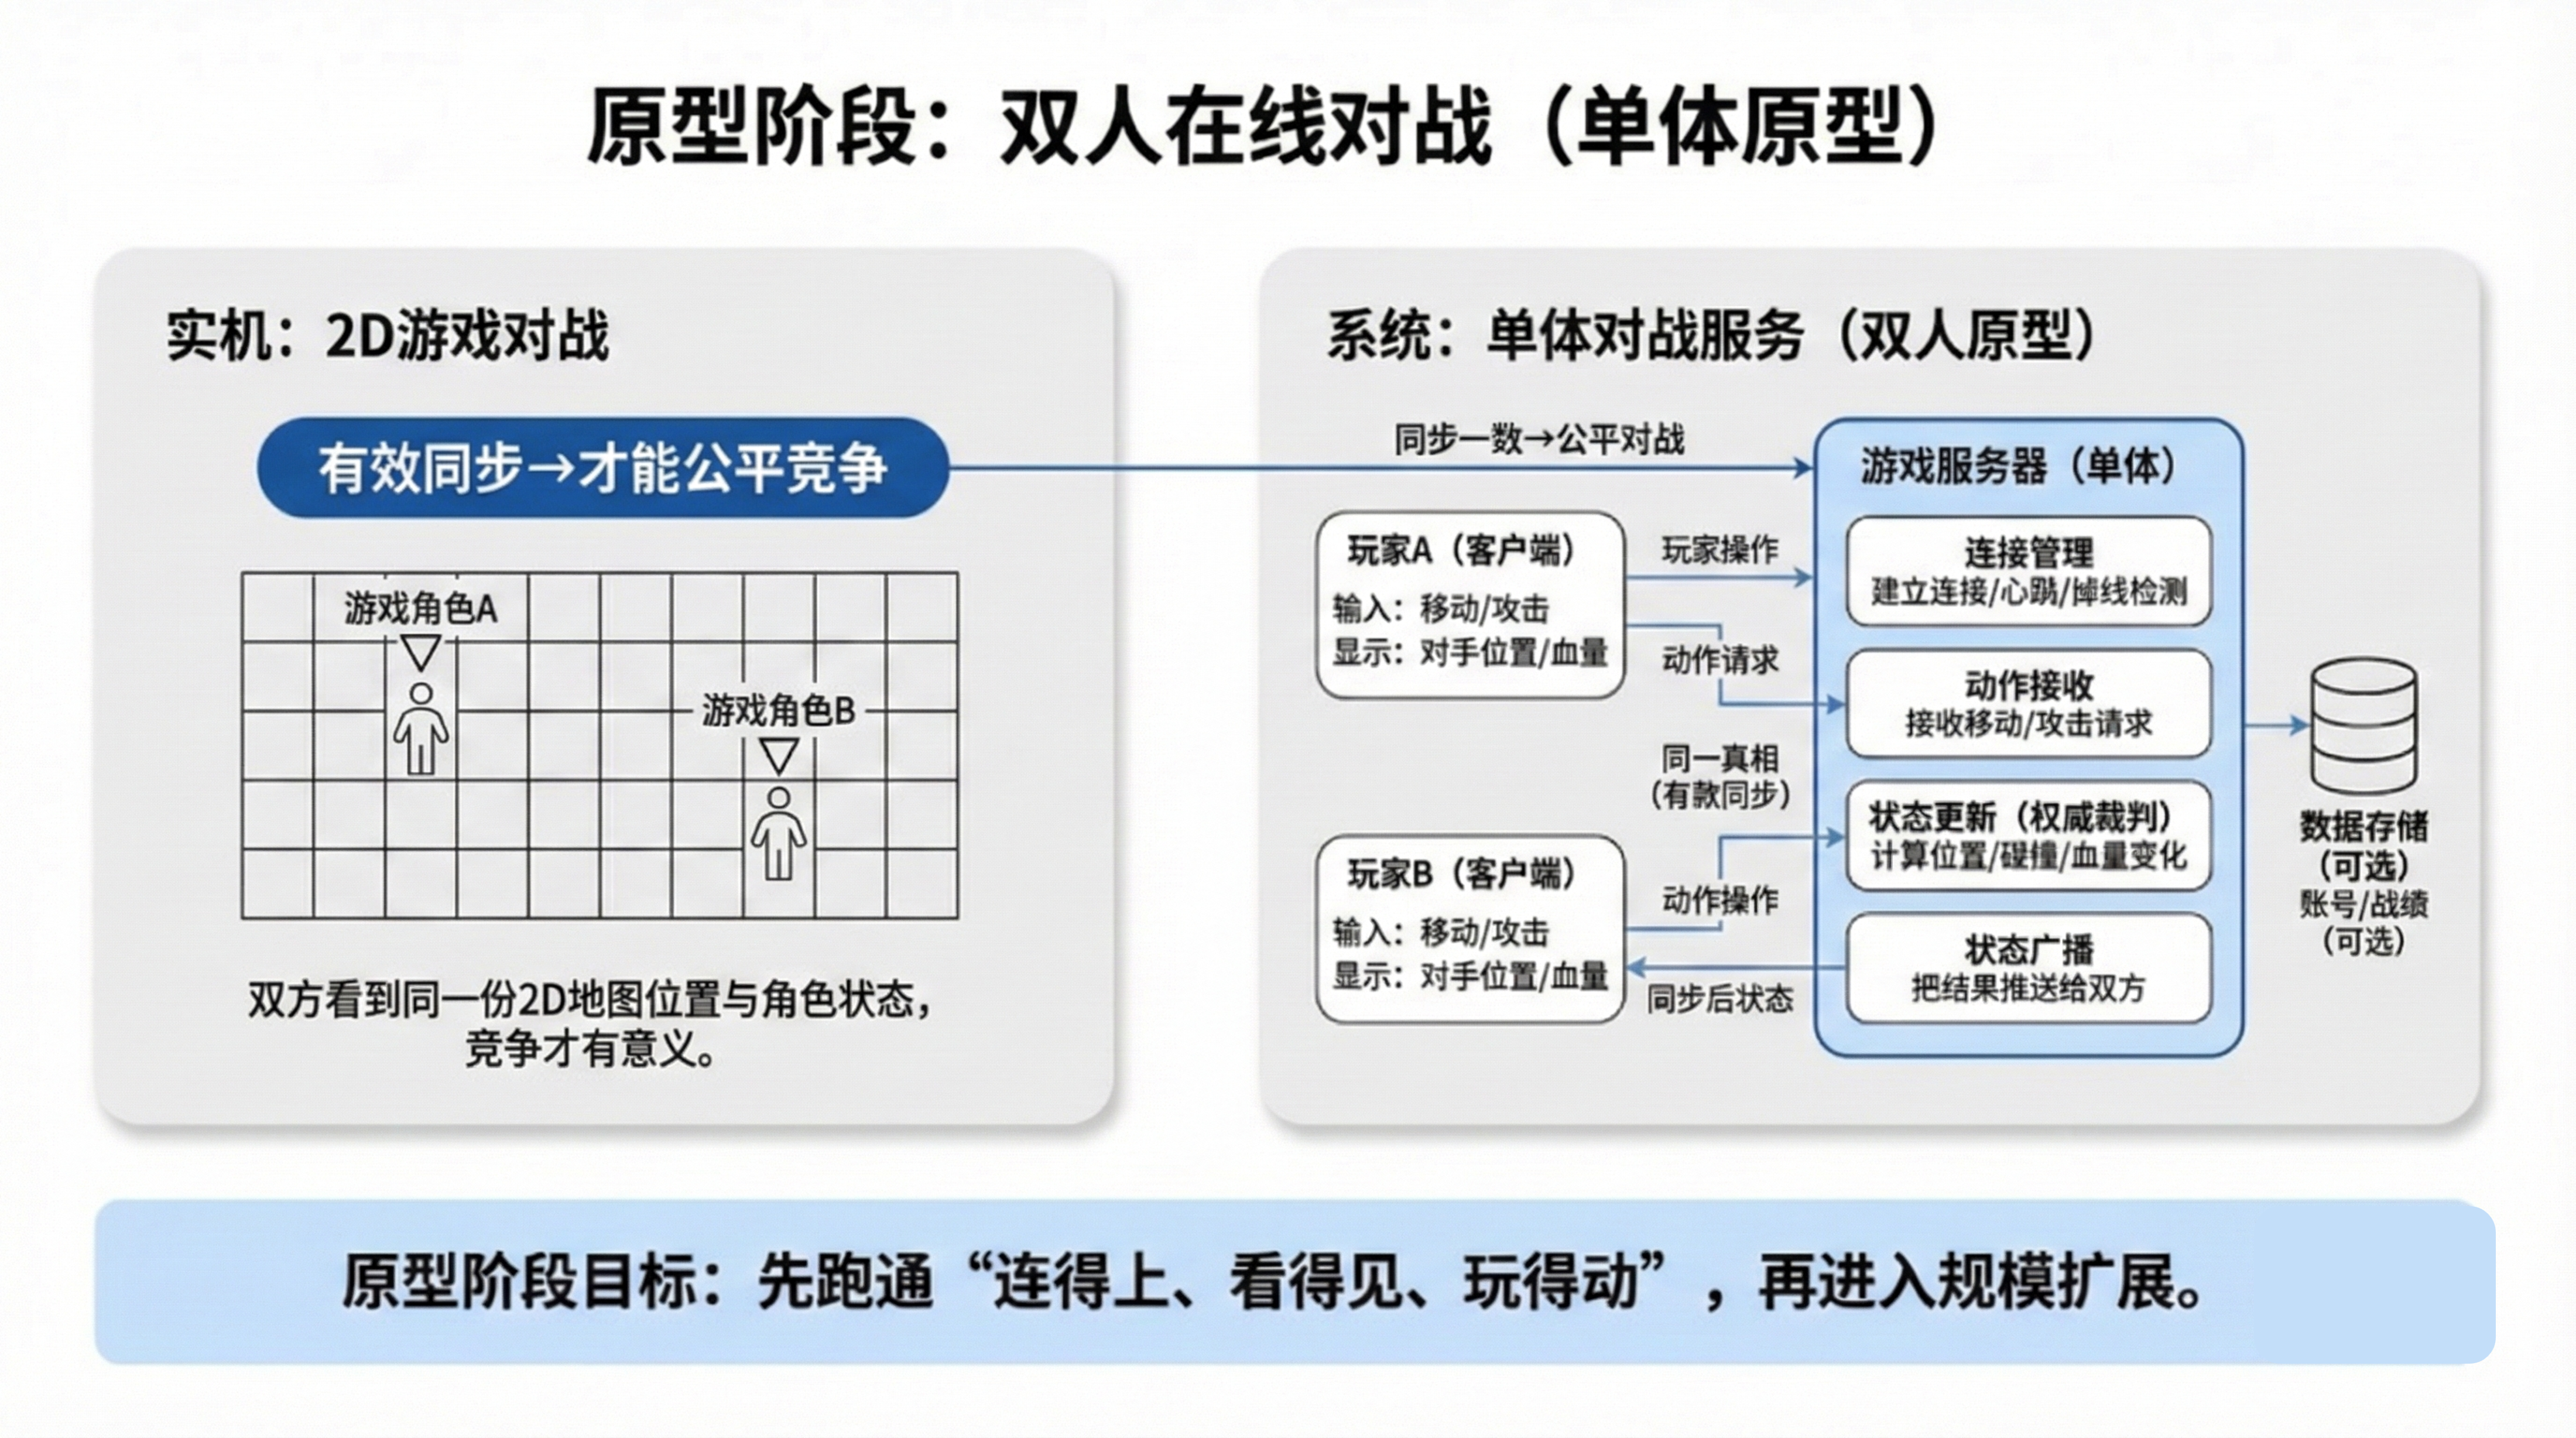
\includegraphics[width=1.0\textwidth]{figures/sec1/intro-phase2-fixed1.png}
    \vspace{-30pt}
    \caption{可竞技的单条跑道与单体架构}
    \label{fig:intro-phase2}
    \vspace{-15pt}
\end{figure*}

如图\ref{fig:intro-phase2}所示，\textbf{原型阶段}的目标是先构建一个最基础在线对战系统。我们基于最典型的“双人同图对局”开始游戏：两位玩家进入同一张地图开始走位、试探，每一次操作都应当在对方视角中及时出现并得到一致的反馈。若双方看到的位置、血量或判定结果不一致，就会立刻产生“我明明打中了/我明明躲开了”的割裂体验，对战也就失去可信的基础。因此，这一阶段关注的核心不是玩法的复杂度，而是把小地图的实时交互闭环跑通，并确保双方始终基于同一份游戏状态进行对抗。

在系统实现层面，我们用一个单体游戏服务器来支撑这一基本闭环。客户端发出动作请求，服务端负责管理连接、接收请求、计算新的游戏状态，并将结果广播回每个客户端。服务器的状态广播就像比赛中的裁判，它确保每一方看到的是相同的状态，从而让两位玩家在游戏过程中感受到实时、可信的反馈。只有把连接、请求、状态更新与同步三个步骤完整跑通，才能保证玩家能“连得上、看得见、玩得动”，为后续面对更多玩家或更复杂业务的扩展打下最基本的工程基础。

进入\textbf{并发优化阶段}后，如图\ref{fig:intro-phase3}所示，交互场景发生了质变：战场不再局限于双人对决，而是瞬间涌入成百上千名玩家。这种高密度的交互使得原有的架构不堪重负，由此产生的操作延迟感、动作变形感会迅速消耗玩家的耐心。映射到系统层面，就是处理请求的速度跟不上玩家请求数的增长，导致卡顿、延迟甚至错误。因此，本阶段的核心任务是精准定位瓶颈，通过在现有架构下进行精细化调优，拓展系统的承载极限，使其在多用户高压环境下依然能保持高效与稳定。

\begin{figure*}[htbp]
    \vspace{-13pt}
    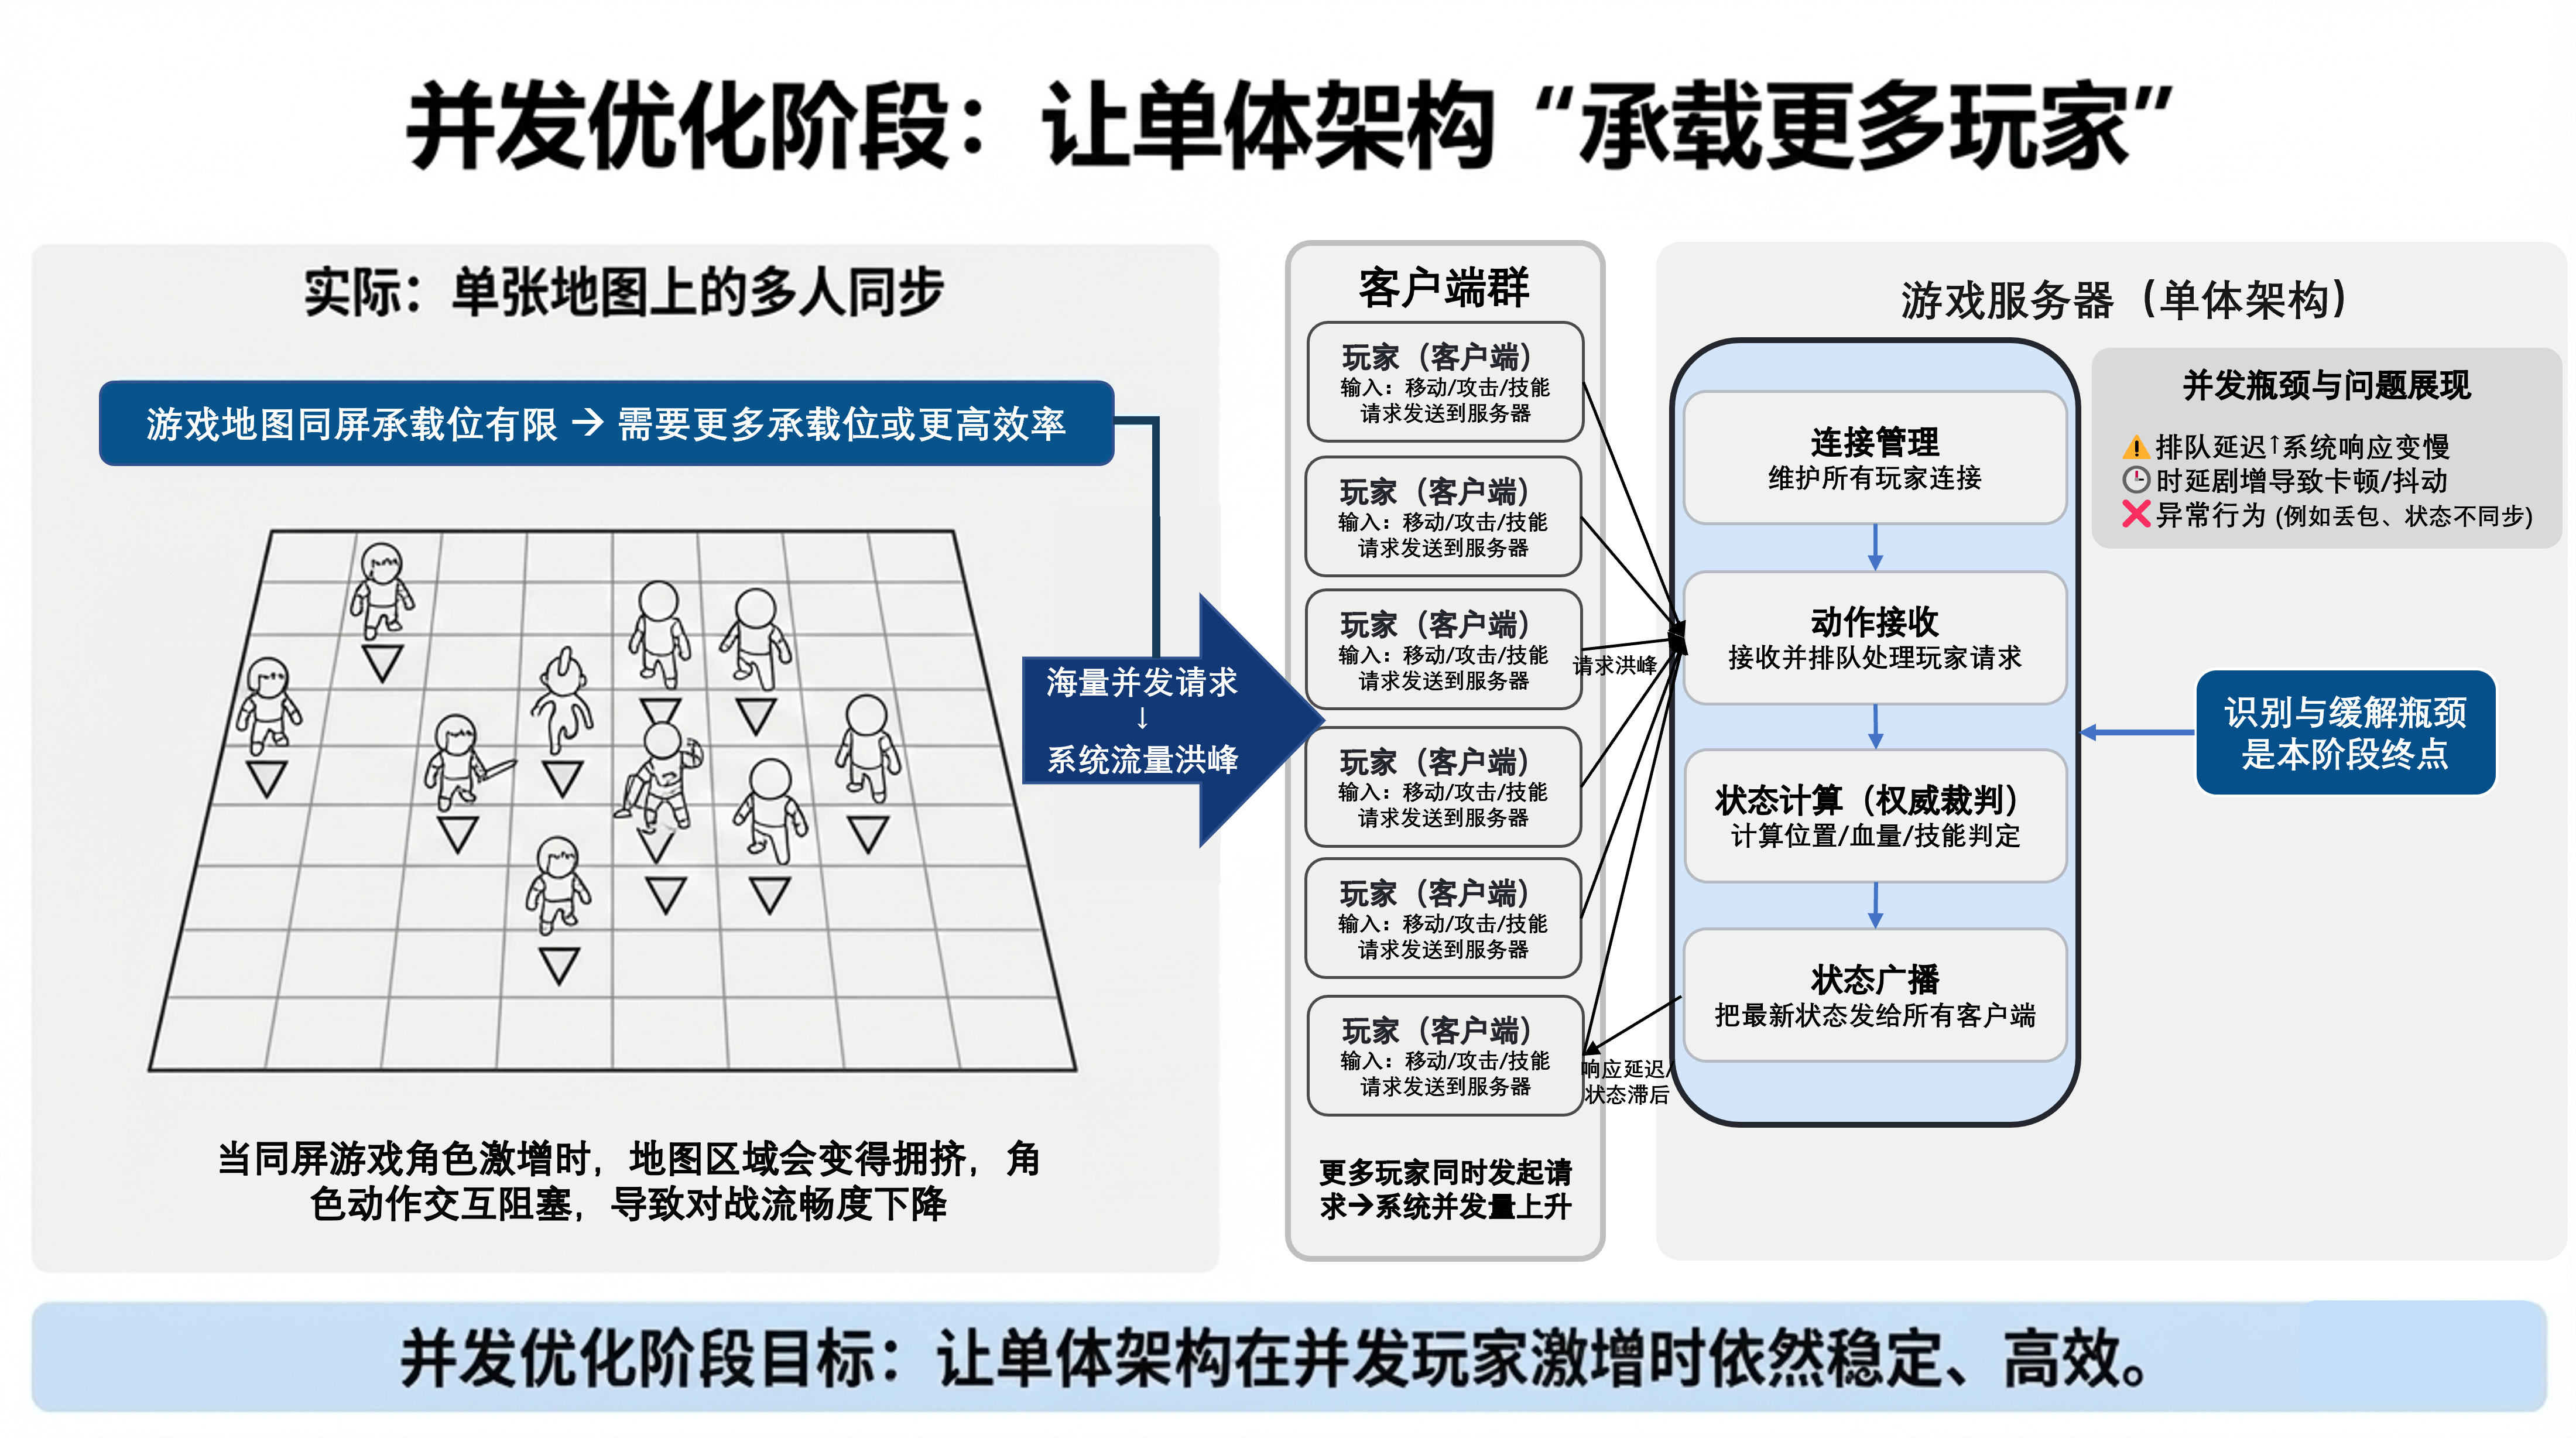
\includegraphics[width=1.0\textwidth]{figures/sec1/intro-phase3-fixed1.png}
    \vspace{-30pt}
    \caption{高性能的单条跑道与并发单体架构}
    \label{fig:intro-phase3}
    \vspace{-15pt}
\end{figure*}

如图\ref{fig:intro-phase4}所示，当同一张地图里的玩家数量持续激增，“把所有人都塞进一张地图”的策略终究会遇到天花板。战场越拥挤，每一次移动或技能释放所引发的同步成本就越高，最终导致系统不堪重负。为了承载更大的规模，我们必须打破单体限制，将在线世界开辟成由多张地图组成的“互联群岛”，这标志着我们正式进入了\textbf{分布式阶段}。在系统中，这意味着将不同功能拆分到多台机器上协同运行，各自处理特定的任务（如登录、对战逻辑、状态同步等），并通过网络协调它们之间的状态一致。对应到系统设计，这意味着不再由一台机器包揽所有工作，而是将登录、逻辑计算、状态同步等任务拆分到不同的机器上协同处理。虽然这种“人多力量大”的模式解决了容量难题，但也带来了挑战：多地图之间如何保持步调一致？如何防止某张地图突然崩溃导致整个游戏不可玩？因此，本阶段我们将以游戏中的跨地图互动为例，带读者理解分布式系统中“协同”与“一致性”的本质，并动手解决这些问题。

\begin{figure*}[htbp]
    \vspace{-13pt}
    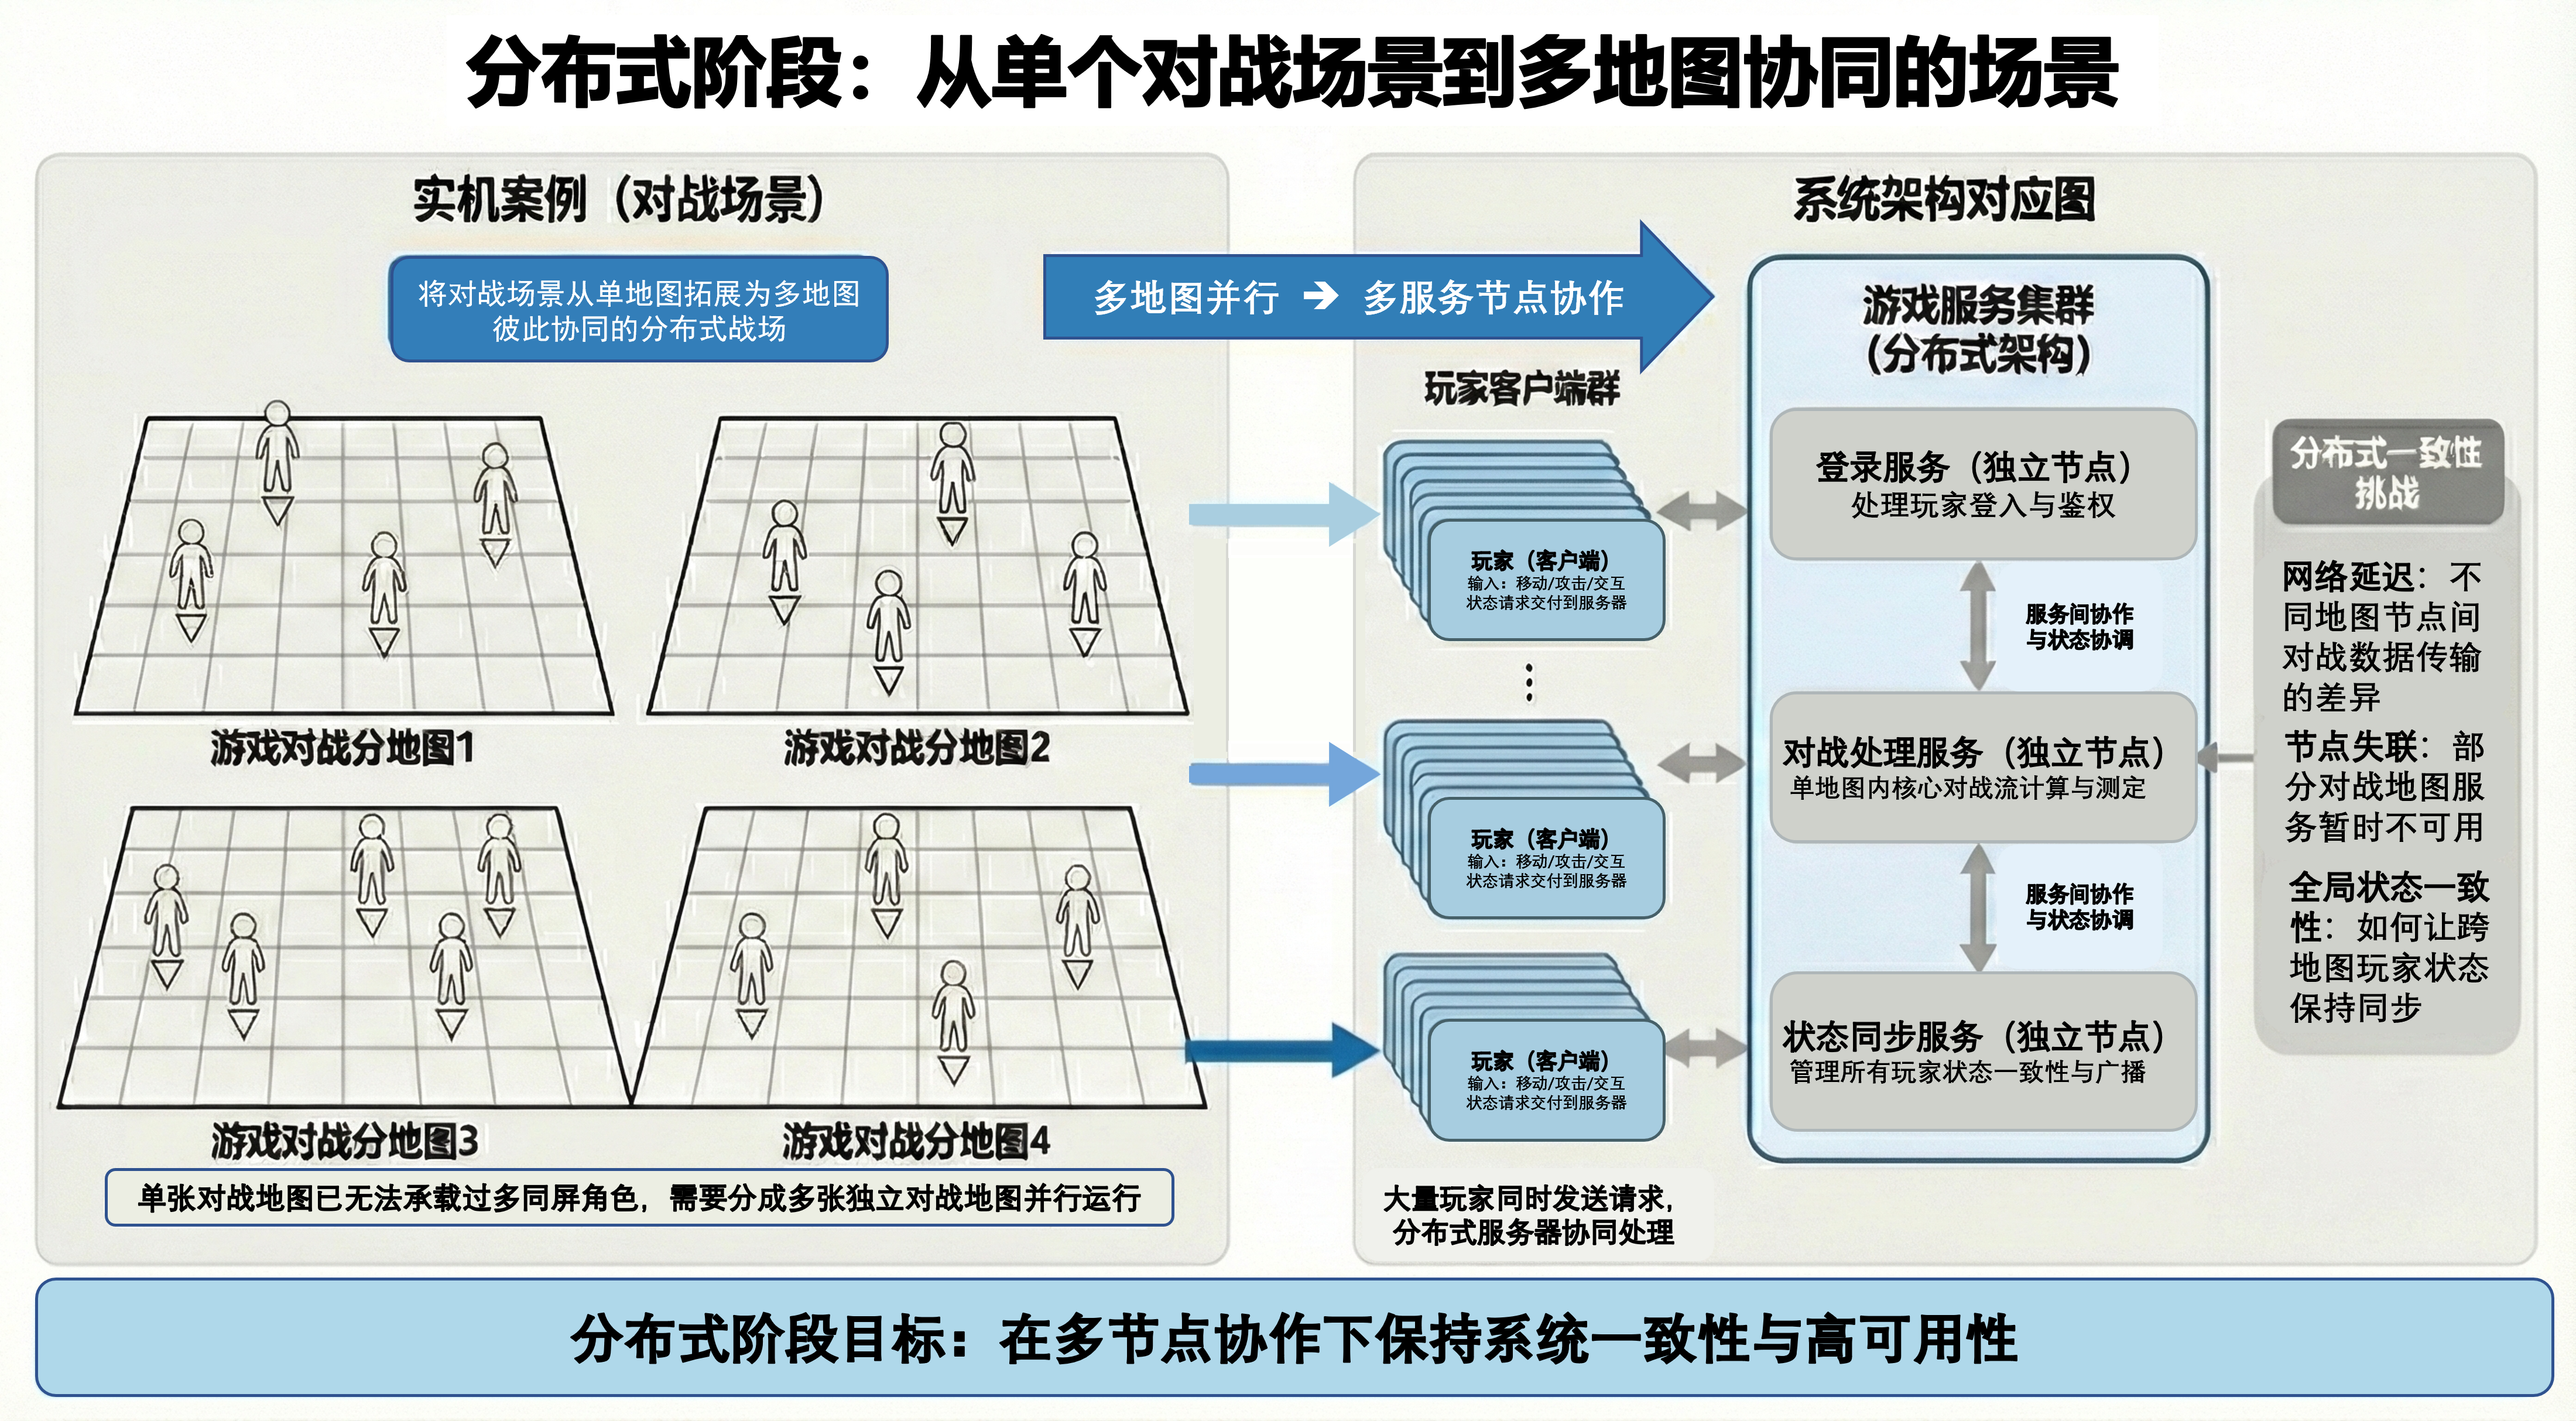
\includegraphics[width=1.0\textwidth]{figures/sec1/intro-phase4-fixed1.png}
    \vspace{-30pt}
    \caption{多跑道与多服务器分布式架构}
    \label{fig:intro-phase4}
    \vspace{-15pt}
\end{figure*}

最终，在\textbf{容器化阶段}，如图\ref{fig:intro-phase5}所示，我们的视角不再局限于手动管理地图，而是升级为对整个“游戏宇宙”的自动化治理。这种能力类似于智能化的副本管理系统：它不再依赖人工去开服合服，而是将服务打包成一个个标准的副本单元（容器）。当玩家蜂拥而至时，系统能瞬间复制出成百上千个平行的副本世界来承载流量；当人潮退去，多余的副本则会被自动回收。对应到技术层面，这正是容器打包与自动化编排的精髓，通过将服务标准化封装，配合编排系统（如Kubernetes）的调度，系统能够根据实时用户数量动态伸缩资源，甚至在某个副本“崩溃”时毫秒级自动重建，无需人工连夜上线救火。这种弹性调度与自动化管理，正是云计算支撑大规模复杂业务的基石。

\begin{figure*}[htbp]
    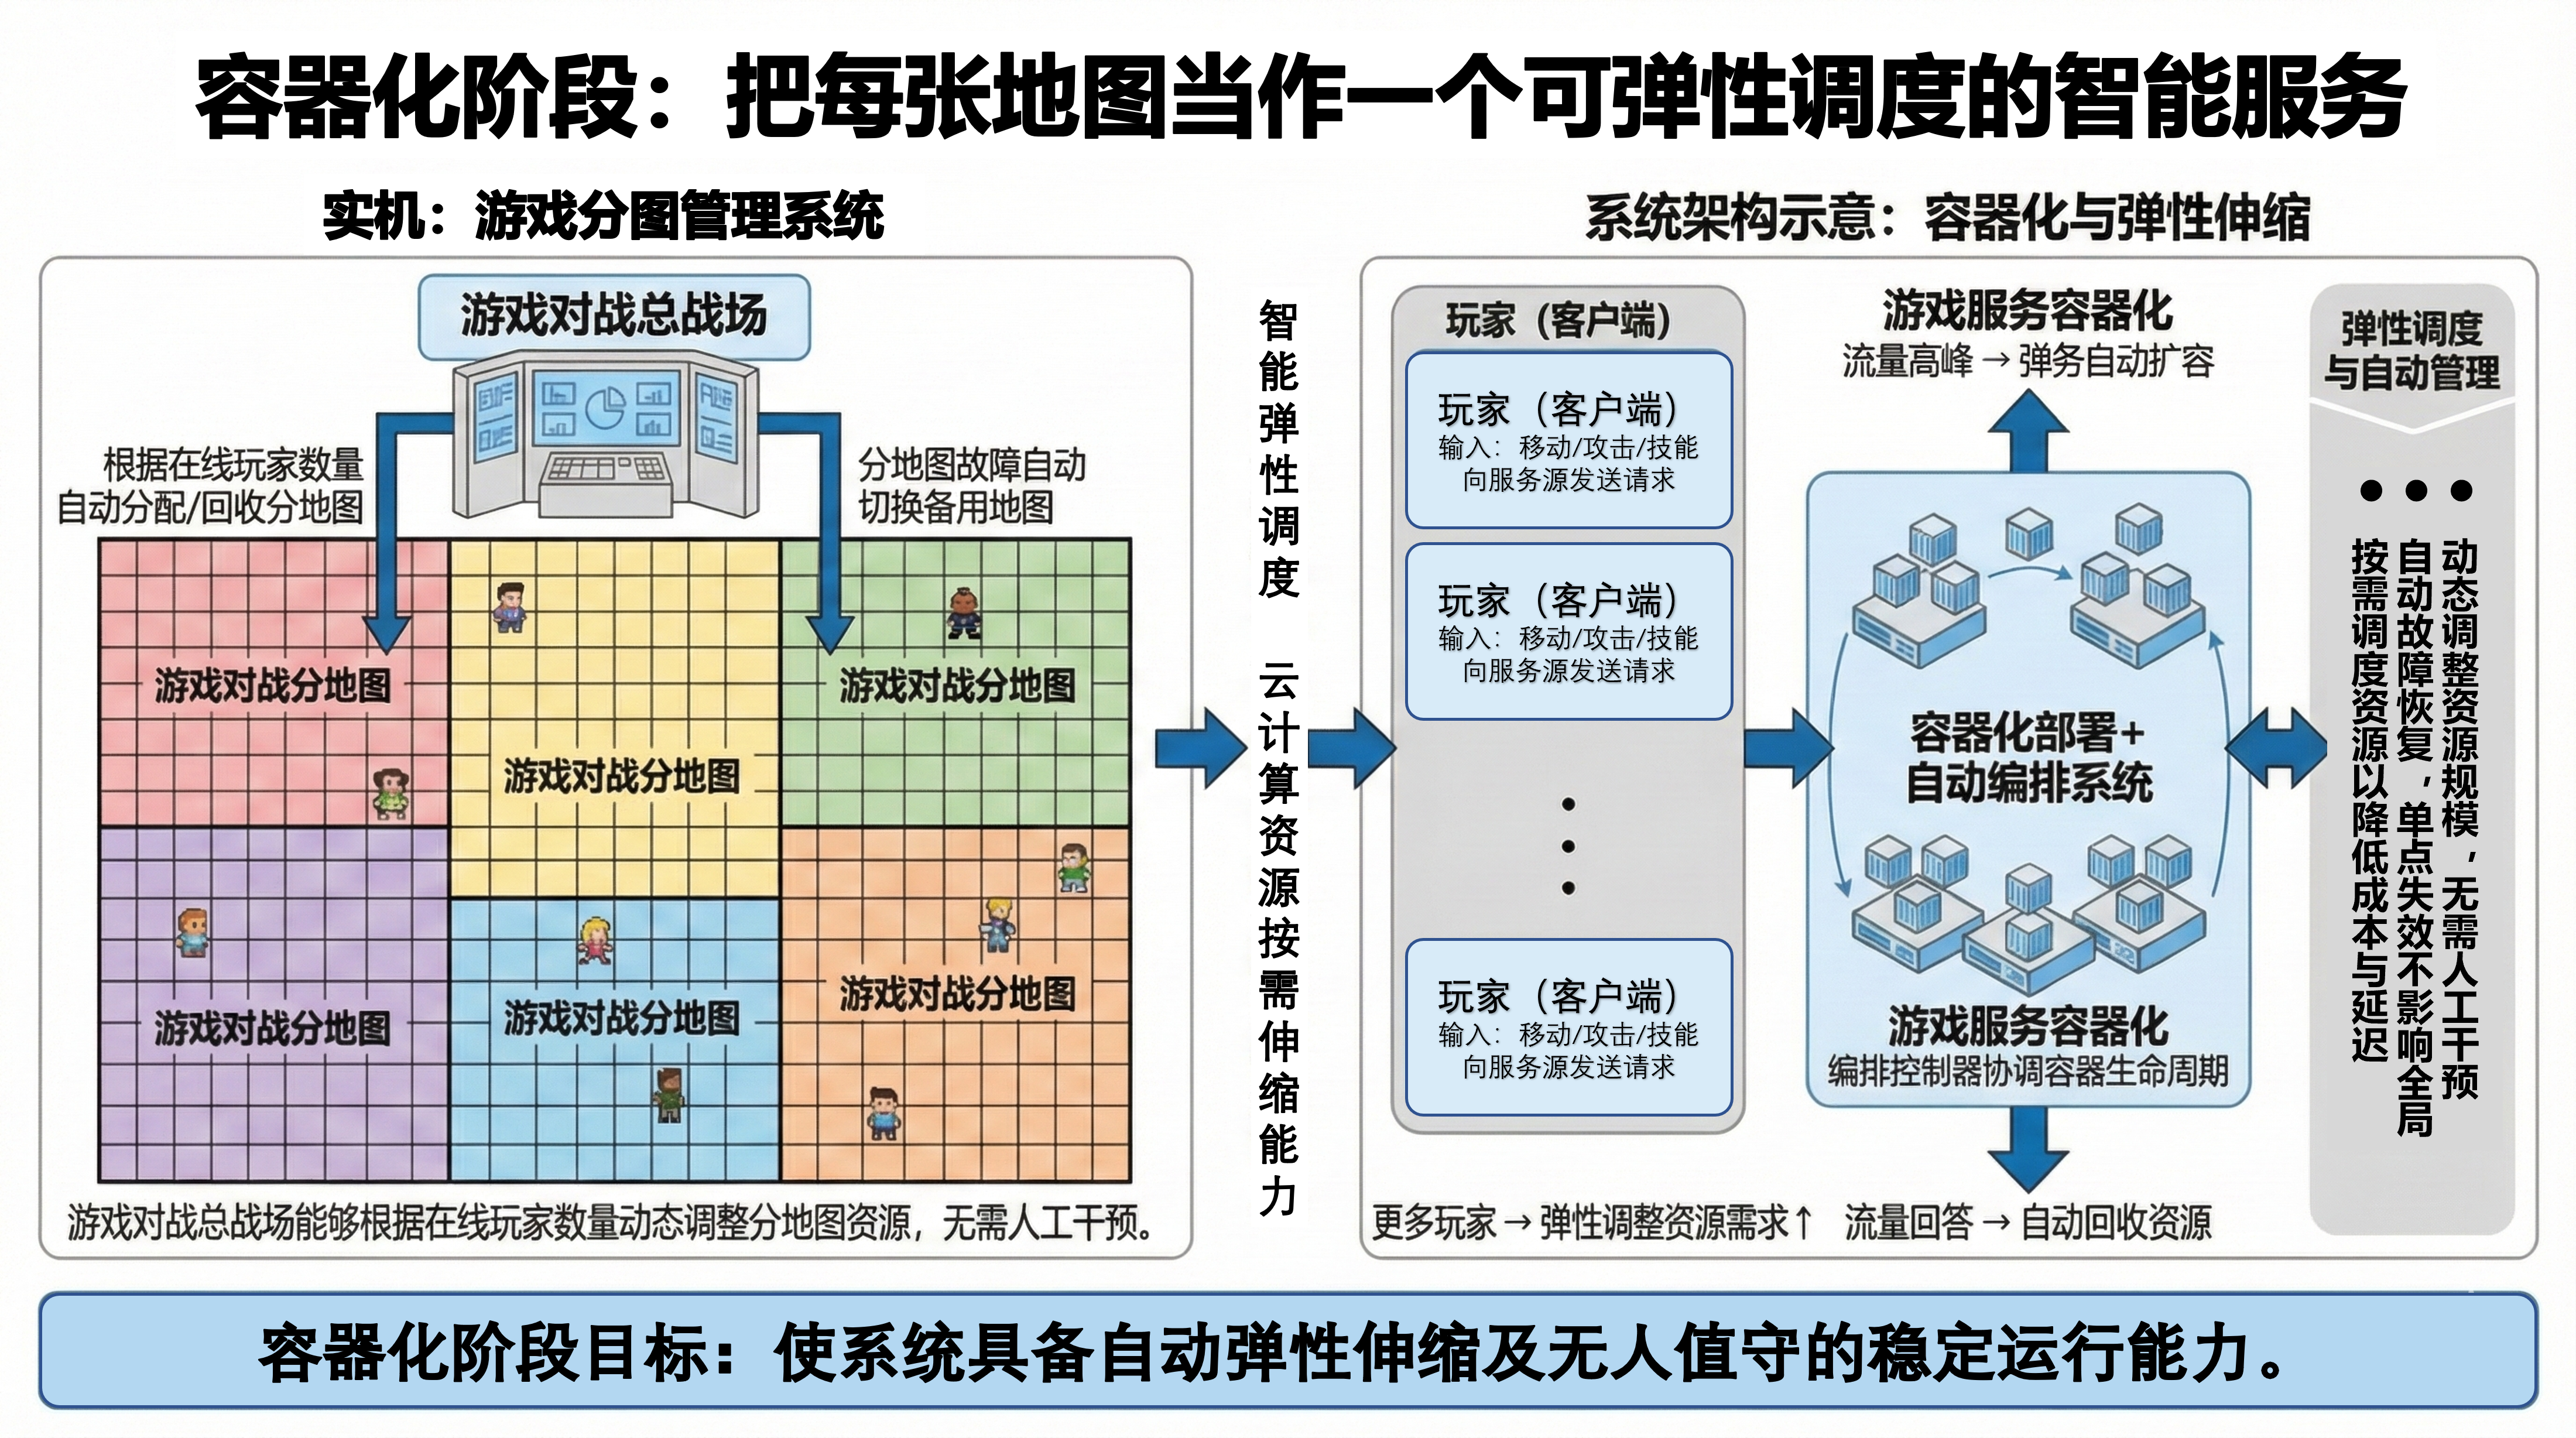
\includegraphics[width=1.0\textwidth]{figures/sec1/intro-phase5-fixed1.png}
    \vspace{-30pt}
    \caption{弹性智能体育场与容器化架构}
    \label{fig:intro-phase5}
    \vspace{-15pt}
\end{figure*}

通过梳理这一系列从单张小地图到分布式群岛，再到弹性平行世界的架构演进，读者不仅能直观地看到系统在不同规模下所面临的特定瓶颈，更能深刻理解每一项技术引入背后的工程必然性。这套演进逻辑清晰地揭示了云计算的核心原理：我们何时需要深挖单机性能，何时必须转向横向协作，又在何种契机下引入弹性扩缩与自动化编排。正是这些能力的层层递进与有机结合，最终支撑起大规模在线服务的稳定运行。




\subsection{神兵利器：搭建游戏开发的“兵工厂”} % 介绍全文的技术设定

\subsubsection{兵工厂的装配线：从闭环到运维的四道工序}
一款多人在线游戏其实是一个长期运行的工程系统，它的核心并不在于某一项具体技术，而在于这些技术如何在前述架构的演进之下被逐步引入、拆解并协同工作。从这个角度看，系统的构建过程更像是在搭建一座兵工厂，我们不能仅仅停留在整体架构的描述层面，而是围绕明确的生产目标，在装配线的不同位置逐步引入并剖析支撑系统运转的关键技术能力。

这条装配线的起点，是建立一个能够稳定产出结果的最小闭环。只有当系统具备明确的裁决规则与一致的状态演化方式，后续的优化与扩展才具有意义。在此基础上，随着负载与规模的增长，系统需要不断引入新的能力来应对性能压力、资源瓶颈与复杂协作需求，而这些能力是沿着既定工序逐步叠加。

从工程视角看，这一演进过程可以被理解为四道连续的工序：先保证交互闭环的正确性，再提升系统在压力下的稳定性，随后扩展到多节点协同，最终引入自动化运维与弹性调度机制。每一道工序的引入，都是对前一阶段能力边界的补充，而不是对既有设计的推翻。

在后续章节中，我们将沿着这条装配线逐步前进，阐明每阶段会遇到的问题以及必须引入的工程能力，并通过具体实现展示这些能力如何共同构成一个可扩展、可维护的在线游戏系统。

\subsubsection{立规矩：权威裁决与消息化交互}\label{sec:权威裁决与消息化交}
多人在线对战的本质，是一场持续进行的规则博弈。只要对战尚未结束，所有参与者就必须接受一个前提：世界中发生的每一次关键事件，都只能有一个被承认的结果。如果玩家可以各自宣布“我已经命中”或“我已经躲开”，那么对战本身便无法成立。因此，当多个玩家通过共同进入同一个游戏世界时，我们系统设计的首要问题便随之出现：在出现分歧的情况下，谁拥有定义结果的权力。

基于这一现实约束，本书在第二章确立了一条最朴素、也最稳固的设计原则：裁决权必须集中，表达权可以分散。在一场在线对战中，所有玩家各自操作着自己的设备，但这些设备并不直接决定世界发生了什么。它们所能做的，只是不断向一台专门负责判定的裁判机器表达“我想要做什么”，例如向前移动、释放技能或发起交互请求。世界是否真的发生了变化、变化以何种方式生效，则完全由这台裁判机器依据统一规则来决定。

在这种分工下，就可以保证裁判机器在自身内部维护着一份完整且连续的世界状态，并以此作为所有判断的唯一依据。玩家设备上看到的画面，始终只是这份状态在本地的呈现。通过将“想做什么”和“最终发生了什么”明确区分开来，系统避免了不同设备各自为真、相互矛盾的情况，使对战能够在不能控制玩家设备的现实条件下依然保持公平与一致。

当我们把裁决交给裁判机器之后，玩家机器与其的配合方式就需要调整。因为玩家设备和裁判机器隔着互联网，彼此看不见对方的内部情况，也不可能像在同一台电脑里那样“直接伸手去改数据”。更稳妥的做法，是把每一次协作都变成一条条说清楚的话：想做什么，就发一条消息告诉裁判机器；裁判机器算完结果，也用一条消息把结论发回来。这样一来，玩家设备做的事情就很简单了，它只负责把操作翻译成请求发出去，然后把收到的结果展示出来。裁判机器只负责按统一规则做判断，再把确认后的结果回传。整个过程就像一问一答，双方都只认“收到的消息”这份证据，因此即使网络有延迟、设备各不相同，也不会出现各自为真、说不清楚的混乱局面。

在这种一问一答的配合方式里，消息就成了双方唯一能对得上的“凭证”，因此消息统一的格式需要精心设计。既然一切都靠消息说话，那么消息就不能随便写，必须有一个大家都能看懂、也不容易写乱的固定格式。否则今天玩家用自然语言发送请求，明天又换成了底层的01数字串，裁判机器为了去读懂就需要不断地进化，系统很快就会因为这些鸡毛蒜皮的小事情而变得难以维护。

最简单也最实用的做法，是让每条消息都包含两部分信息：第一部分说明“这条消息在说什么”，也就是它属于哪一类请求或哪一类结果；第二部分说明“这次要说清楚需要哪些细节”，例如是谁在操作、具体做了什么、发生在什么时间点。这样一来，双方看到消息的第一眼就能知道该走哪条处理流程，再从后面的细节里取出需要的数据完成判断或展示。只要这个格式保持稳定，我们就可以在不影响已有功能的前提下逐步增加新的交互类型，让系统在功能变多时依然保持清晰可控。在附录D中，我们会对“消息格式”统一的工程化问题进行进一步的探讨。

在第二章里，我们会把双人联机原型真正搭起来，把“应该这样设计”的想法落到可运行的系统上，一端把玩家操作整理成请求发出去，另一端集中做判断、更新那份统一的世界状态，再把确认后的结果回传。围绕这条最小闭环，我们会把玩家机器和裁判机器之间的连接打通、裁判机器的基本判定讲清楚以及状态同步实现出来，让读者从抽象概念走进可验证的工程现实，并为后续章节在同一骨架上继续扩展能力打下基础。

\subsubsection{提速稳产：并发与延迟控制}\label{sec:并发与延迟控制}
在第二章把双人对战跑通之后，我们马上会遇到一个现实且棘手的问题：当房间里不仅仅是两个人，而是成百上千人同时在线时，裁判机器还能不能反应得过来？在双人场景下，裁判机器只需要面对两个玩家机器的请求，哪怕它是慢条斯理地按先来后到的顺序一个个处理，玩家也不会觉得卡顿。但当同一张地图里涌入大量玩家，无数的移动、攻击、施法请求像潮水一样涌向裁判机器。此时，如果依然坚持“一次只做一件事”，后来的请求就会在裁判机器门口排起长队，队伍越排越长，玩家感受到的延迟也就越来越高，最终导致游戏体验崩盘。

第三章的核心任务，就是教会裁判机器学会“一心多用”，也就是编程领域常说的“并发”。并发并不是让机器的计算速度在物理上变快，而是通过一种巧妙的时间管理技术，让它在同一秒钟内同时推进几十甚至上百个玩家的请求。我们会引入 Go 语言特有的“轻量级线程”（Goroutine），这就像是给每一位进入游戏的玩家都配备了一名专属的服务员。这样一来，无论来了多少客人，大家的需求都能被即时响应，而不需要都在同一个窗口前苦苦等待。

然而，一旦开启了并发模式，新的麻烦随之而来。当成千上万个服务员同时在读写同一份世界数据时，冲突在所难免。想象一下，两个玩家几乎同时冲向地图上唯一的一把宝剑，两个服务员都判定自己的玩家捡到了，结果就是一把剑被“复制”成了两把；或者两个人同时攻击一只怪物，本来应该扣两份血，却因为写入冲突只扣了一份。这种因“手忙脚乱”导致的数据错误，在技术上被称为“竞态条件”，它是并发模式中最容易导致游戏逻辑崩溃的杀手。

为了解决这种混乱，我们需要引入“锁”的机制。锁就像是试衣间的门，当一个服务员正在修改某个关键数据（比如怪物的血量或宝箱的状态）时，他必须先锁上门，此时其他试图修改同一数据的服务员只能在门外排队等待。虽然这看起来似乎又回到了排队的老路，但因为计算机处理单个修改的速度极快，这种微秒级的等待人类根本察觉不到。第三章将详细讲解如何精准地使用这把锁，既要锁住关键数据保证安全，又不能锁得太多导致效率低下。

在解决了“快”与“稳”的矛盾后，我们还需要考虑系统的耐久度。频繁地创建和销毁服务员以及频繁地建立与玩家机器的连接，对裁判机器来说都是极大的消耗。为了不让其在长时间运行后因为资源耗尽而“过劳死”，本章还将介绍“池化技术”。这就像是把用过的餐具洗净回收而不是直接扔掉，我们通过建立连接池和对象池，循环利用已有的资源。这不仅大大降低了裁判机器的负担，也让它在面对突发的人数暴涨时，依然能保持稳如泰山的性能表现。

综上所述，第三章是一个分水岭。在此之前，我们是在做一个能跑的“玩具”；而在此之后，通过并发模型、锁机制与资源复用的组合拳，我们将构建出一个真正具备工业级强度的游戏引擎核心。它不再畏惧海量并发，能在一个严守秩序的平行世界里，为成千上万名玩家提供丝般顺滑的实时对战体验，也为后续章节向分布式架构的演进打下了最关键的单机性能基础。



\subsubsection{扩建分厂：服务拆分与多机协作及一致性权衡}\label{sec:服务拆分与多机协作及一致性权衡}
把第三章的并发问题解决后，单台裁判机器虽然能更加眼疾手快地处理请求，但它的脑容量（内存）和计算能力（CPU）毕竟是有上限的。当游戏地图大到无边无际、玩家多到成千上万时，累死一台机器也忙不过来。这时候，唯一的办法就是“扩建分厂”，不再让一台机器死扛所有压力，而是把巨大的游戏世界切成很多块，每一块区域都派一台专门的裁判机器去管理。第四章要讲的就是如何让这一群裁判机器不仅各司其职，还能配合得像一个人一样默契。

把世界切开很容易，难点是切开后还要让玩家感觉不到缝隙。这就好比两位裁判分别管理地图的左半边和右半边，当玩家站在中间的分界线上时，他必须能一眼看到对面的情况。如果机器之间互不通气，玩家就会看到世界在脚下突然断掉了。为了解决这个问题，我们需要教会裁判机器互相“传话”，把对面发生的景象实时投影过来，就像在边界上放了一面镜子，让玩家即使身处不同的管理区域，也能感受到一个完整、连续的世界。

看得见只是第一步，更麻烦的是动手。如果站在左边的玩家，向站在右边的玩家扔了一块石头，这块石头到底砸没砸中，该由哪边的裁判说了算？左边的裁判管不了右边的人，右边的裁判又不知道左边什么时候扔的石头。如果两边各执一词，游戏就会乱套。这一章我们会制定一套“跨界办事”的规矩，明确在两个人跨越地盘打架时，到底谁才是临时的“主裁判”，确保这种复杂的纠纷也能被公平地解决。

除了打架，玩家还会经常在地图之间来回穿梭。当玩家从左边走到右边，就不只是简单的移动了，这在后台意味着他要把自己的全部家当如等级、装备、血量等，从一台机器的里搬家到另一台机器里。这个过程就像在海关办理交接，必须严丝合缝。如果这边刚把人注销了，那边还没来得及登记，玩家的数据可能就会瞬间“蒸发”。我们会通过具体的案例，演示如何设计一套安全的“交接仪式”，保证玩家无论怎么跑，数据都丢不了。

既然变成了多台机器一起工作，我们还得面对一个更倒霉的情况：万一其中一台机器突然坏了怎么办？在单机时代，机器坏了世界就停了；但在集群里，不能因为一个分厂停电就让整个世界崩塌。我们需要从之前单纯依赖机器脑子里的记忆（内存），转变为把重要的事情记在这一本公共的“史书”（日志）上。这样一来，通过这本谁都赖不掉的账本，我们就能在机器出问题时把数据找回来，或者让其他机器顶替它的工作。

第四章的内容，我们会实现从“单机应用”到“分布式集群”的关键架构质变。通过这一章的学习，你将掌握如何利用多台物理服务器构建一个支持横向扩展的工业级系统，这是对分布式数据一致性、跨进程通信以及容错机制的深度实践。攻克了这些技术难题，意味着我们的系统不再受限于单机的性能瓶颈，真正具备了支撑海量用户与无限地图的工程底座，这也标志着你的服务端架构设计能力正式迈入了大流量、高并发的专业领域。


\subsubsection{调度中枢：容器化、编排与弹性运维}\label{sec:调度中枢}
当我们将游戏世界的逻辑在代码层面打通，并设计好了多机协作的规则后，面临的下一个挑战是如何让这就庞大的系统真正“跑”起来。在开发阶段，我们往往会遇到一个经典难题：代码在程序员自己的电脑上跑得好好的，一发布到服务器上就报错。这是因为不同的机器就像装修风格迥异的厨房，有的缺佐料，有的锅灶型号不对。第五章首先要解决的就是这个“水土不服”的问题。我们将引入“容器化”技术，这就像是把我们的游戏代码、数据库以及它运行所需的一切环境，全部打包进一个标准化的“集装箱”里。无论把这个箱子运到哪台服务器上，只要打开箱子，里面的运行环境都是一模一样的，彻底告别了“在我电脑上明明没问题”的尴尬。

有了“集装箱”，我们发货是方便了，但一个完整的游戏大区往往需要几十甚至上百个这样的箱子配合工作——有的负责存数据，有的负责算战斗，有的负责管登录。如果靠人工一个个去启动、去连线，不仅效率低，还容易接错线。因此，我们需要一位能看懂图纸的“工头”。因此，我们将学习如何为多个“容器”编写一份简单的“编排清单”，告诉它们要开几个战斗服、几个匹配服，它们之间该怎么连接。有了这份清单，哪怕面对复杂的服务器集群，我们也只需要敲一行命令，系统就能自动把整个游戏大区像搭积木一样瞬间搭建起来。

然而，真正的考验往往发生在游戏上线之后。服务器就像不知疲倦的工人，但工人也会生病，机器也会宕机。如果半夜三更有一台负责核心战斗的服务器突然坏了，难道要运维人员从被窝里爬起来去重启吗？这就需要引入更高级的“云端指挥官”——Kubernetes。它像是一个拥有上帝视角的管家，24小时盯着所有服务器的状态。一旦发现某个机器“坏掉”了，它会在几秒钟内自动在另一台健康的机器上重新启动一个一模一样的替补，确保玩家几乎感觉不到故障的发生。这种自我修复的能力，是现代大型在线游戏保持永不掉线的秘诀。

除了应对故障，“指挥官”的另一大本事是应对流量的潮汐。游戏人数在一天中是波动的，周五晚上的玩家可能比周二上午多出十倍。如果服务器的数量固定不变，要么在高峰期把玩家堵在门外，要么在低谷期白白浪费机器租金。我们随后还会揭示“弹性扩容”的奥义：教会系统根据实时的玩家人数自动调节规模。人多了，自动租新的机器加入集群；人少了，自动释放多余的机器帮老板省钱。这种能屈能伸的架构，才算得上是真正“活”在云端的现代化系统。

通过第五章的学习，我们的视角将从写代码的微观逻辑，升级到掌控整个服务器集群宏观运维。你将不再仅仅是一个能写出好玩游戏的程序员，更将进化为一名能够驾驭云端算力、指挥千军万马的云原生系统架构师。至此，从单机逻辑到分布式协作，再到云端的自动化运维，本书将帮你完成游戏服务端开发全链路的技术闭环。

\subsection{技术选型与全栈图谱}

在前文中，我们已经从系统演进的角度，勾勒了一条从最小闭环到弹性集群的工程路径，并将这一过程类比为一条逐步完善的“兵工厂装配线”。然而，任何装配线都必须落在具体的材料与工具之上，否则架构设计只会停留在抽象层面。

本节的目标，正是将前述的设计原则与演进思路，映射到一套可落地、可实现、可扩展的云计算技术栈上。从工程视角看，一个现代云计算项目并非由单一技术构成，而是由计算节点、通信机制、数据存储与基础设施协同组成的系统整体。不同层次的技术承担着不同的职责，它们共同决定了系统在性能、可靠性与可维护性上的上限。

从系统边界来看，一个典型的云计算项目由三类核心要素构成：对外提供服务的交互入口、支撑业务逻辑的数据治理体系，以及承载系统运行的基础设施层。这三者相互配合，共同决定了系统的性能上限、可靠性与可扩展性。如图 \ref{fig:architecture} 所示，本书采用的技术架构遵循现代高并发在线系统的通用范式，并为后续从单体原型演进至云原生集群预留了充分空间。

\begin{figure*}[htbp] 
\centering 

\includegraphics[width=0.8\linewidth]{figures/sec1/architecture.png} 
\caption{项目整体技术架构图} 
\label{fig:architecture} 
\end{figure*}

\subsubsection{交互中枢：CS架构与权威裁决}\label{subsubsec:cs_arch}

在\ref{sec:权威裁决与消息化交}中，我们已经从功能视角讨论了系统中各类能力模块的组织方式。然而，当这些能力需要被大量终端同时调用，并且直接影响系统的关键状态时，问题的核心便不再是单个模块如何实现，而是系统整体应当如何组织交互与裁决权。

当一个云计算项目需要同时服务大量终端时，首要挑战并非计算能力的不足，而是交互模式与决策机制的设计。在分布式环境中，若每个终端都被允许独立修改关键状态，那么系统将不可避免地陷入状态冲突、逻辑分歧以及一致性失效等问题，这在涉及资源分配、规则执行或竞争行为的场景中尤为致命。

正因如此，现代在线系统普遍采用客户端–服务器（Client–Server，CS）架构作为其基础交互模型。该架构以中心服务器作为权威节点，所有关键业务逻辑与状态裁决均集中在服务器侧完成，而客户端仅作为用户交互入口与结果展示终端存在。其核心思想可以概括为：裁决集中，展示分散。

在 CS 架构下，服务器负责维护系统的“真实状态”，包括业务规则的执行、状态变更的合法性校验以及最终结果的确认；客户端则负责采集用户输入，并将其封装为请求发送给服务器，同时接收服务器返回的裁决结果并加以呈现。这种明确的职责分离，使系统即便面对终端异构、网络延迟或不稳定等现实条件，仍能够保证整体行为的一致性、可控性与安全性。

为了支撑高并发请求与实时响应需求，本书选用 Go 语言构建服务端核心逻辑。Go 语言提供了原生的并发模型（Goroutine）与高效的调度机制，使服务端能够在有限的硬件资源下同时处理大量并发连接，非常适合作为云计算项目中承担裁决与交互中枢职责的实现语言。

客户端与服务器之间的协作，依赖于稳定且可扩展的通信协议。尽管底层网络传输以字节流形式存在，但在业务层面，系统需要一种结构清晰、语义明确的消息格式作为通信契约。为此，本书采用类似 JSON 的结构化消息进行交互，其基本形式如示例所示（详见附录 D）。通过在消息中显式区分“类型”与“载荷”，系统能够在不破坏既有功能的前提下持续演进通信协议，从而有效降低系统演化过程中的耦合度。

\begin{tcolorbox}[title=统一消息格式]
\begin{verbatim}
{
  "type": "MESSAGE_TYPE",
  "payload": {
    // 具体消息内容
  }
}
\end{verbatim}
\end{tcolorbox}

图 \ref{fig:cs_structure} 展示了 CS 架构中客户端与服务器之间的职责分工与交互关系。

\begin{figure*}[htbp] 
\centering 
\includegraphics[width=0.8\linewidth,keepaspectratio]{figures/sec1/chapter1_CS_structure.png} 
\caption{CS架构职责交互示意图} 
\label{fig:cs_structure} 
\end{figure*}

\subsubsection{数据治理：冷热分离存储策略}\label{subsubsec:data_strategy}

在任何云计算项目中，数据都是最核心、也是最复杂的资产。在\ref{sec:服务拆分与多机协作及一致性权衡}，我们已经从功能角度描述了系统所需的各类能力模块，但这些能力最终都必须以数据的形式被记录、查询与更新。换言之，数据层不仅是功能模块的支撑基础，也是系统正确性与可扩展性的最终落脚点。

然而，并非所有数据都具有相同的访问特征与可靠性要求。如果对不同性质的数据强行采用统一的存储方案，系统往往会在性能、成本与安全性之间被迫妥协：要么为了持久化牺牲响应速度，要么为了低延迟承受不可接受的数据风险。

基于这一现实，本书采用冷热分离的数据治理策略，如图 \ref{fig:database_layer} 所示，将系统中的数据按访问频率与重要程度划分为不同层次，并分别选择最合适的存储技术加以承载。

\begin{figure*}[htbp] 
\centering 
\includegraphics[width=0.8\linewidth,keepaspectratio]{figures/sec1/chapter1_database.png} 
\caption{服务端的数据存储分层} 
\label{fig:database_layer} 
\end{figure*}

一类数据具有“高频读写、强实时性、短生命周期”的特征，例如会话状态、实时计算结果或临时中间态。这类数据通常直接参与交互逻辑，对延迟极为敏感，但又往往可以通过重算、状态同步或回滚机制进行恢复，因此在极端情况下允许发生短暂丢失。针对这类“热数据”，本书选用 Redis 作为内存数据库。

Redis 是一个开源的内存数据库，其核心优势在于将数据存储于内存中，从而提供极低的访问延迟与极高的并发处理能力。它支持多种数据结构，如字符串、哈希、列表、集合和有序集合，并提供原子操作与轻量级事务，能够有效保证高频状态更新过程中的一致性。虽然 Redis 以性能优先为设计目标，但其提供的持久化机制仍可在异常情况下提供基本的数据保护。可以将 Redis 理解为系统的“高速缓冲层”，它承载的是对实时性要求最高、但对长期可靠性要求相对较低的数据。

与之相对，另一类数据则具有“低频更新、强一致性、长期保存”的特征，例如用户账户信息、配置数据或关键业务记录。这类数据的首要目标并非访问速度，而是持久性与正确性，必须在系统崩溃、重启甚至节点迁移后仍然保持完整可靠。针对这类“冷数据”，本书选用 PostgreSQL 作为关系型数据库。

PostgreSQL 是一种成熟的开源关系型数据库系统，以持久化存储与事务一致性为核心设计目标。它支持标准 SQL 查询、多表关联、索引和复杂约束，适合管理结构化且高度关联的数据。同时，其完善的事务机制（ACID）与写前日志（WAL）能够在高并发环境下有效保证数据的一致性与持久性。在云计算项目中，诸如账号信息、任务进度与历史记录等数据访问频率相对较低，但一旦丢失将带来严重后果，因此必须依托 PostgreSQL 这类以可靠性为优先的存储系统进行管理。

通过将 Redis 与 PostgreSQL 进行明确分工与协同使用，系统得以在同一架构下同时满足“快速响应”与“可靠存储”这两类看似冲突的工程目标。这种冷热分离的存储策略，使数据层能够像\ref{sec:服务拆分与多机协作及一致性权衡}所描述的“兵工厂”一样，为上层功能模块提供稳定而高效的支撑，而不成为系统性能或可靠性的瓶颈。

\subsubsection{云端底座：容器化与弹性编排}\label{subsubsec:cloud_native}

在\ref{sec:调度中枢}中，我们已经讨论了系统功能模块的设计与能力划分，但这些模块在实验环境中可以独立运行，并不意味着它们在生产环境中能够稳定、可扩展地部署。随着服务从原型阶段走向真实用户场景，新的工程挑战随之而来：如何在不同机器、不同环境中稳定运行同一套服务？如何在负载波动时快速扩展或回收资源？这些问题已经超出了单纯代码层面的范畴，进入基础设施与运维领域。

为解决“在我电脑上能跑，在服务器上就报错”的环境一致性问题，本书引入 Docker 容器技术。Docker 通过将应用程序及其依赖环境一起打包，提供了一个轻量、可移植且一致的运行环境。无论在开发机、测试环境还是生产服务器中，容器都能以完全相同的方式运行，从根本上消除了环境差异带来的部署风险。容器启动速度快、资源占用低，使游戏服务能够在高峰期迅速“拉起”新的实例应对流量激增。通过 Docker 镜像，我们可以将游戏程序及其依赖库、配置文件打包成标准化单元，实现模块化部署和快速复制，为系统的水平扩展奠定基础。

然而，当服务实例数量从个位数增长到数十乃至数百时，单纯依靠人工管理容器已不现实。此时，系统需要一个自动化平台来统一调度、监控和管理容器实例。为此，本书引入 Kubernetes（K8s） 作为编排系统。Kubernetes 能够持续监控服务运行状态，在实例或节点出现故障时自动完成替换，并根据系统负载动态调整实例数量，实现弹性伸缩。同时，其内建的服务发现与负载均衡机制能够稳定地将外部请求分发到健康的服务实例上，从而在高可用性与资源利用率之间取得平衡。图 \ref{fig:cloud_infra} 展示了基于容器与编排系统构建的云原生基础设施结构。

\begin{figure*}[htbp]
    \centering
    
\includegraphics[width=0.8\linewidth,keepaspectratio]{figures/sec1/chapter1_cloud_docker_k8s.png}
    \caption{云平台的搭建}
    \label{fig:cloud_infra}
\end{figure*}

通过容器化与自动化编排，系统不再依赖人工运维单台机器，而是具备了自我修复、弹性伸缩与负载自适应能力。结合\ref{sec:调度中枢}所描述的模块化设计，云端底座使各功能模块能够以标准化、可复制的方式在大规模分布式环境中落地运行，从而保证系统在用户量持续增长和负载波动情况下仍能保持稳定。Docker + Kubernetes 的组合不仅降低了运维复杂度，还释放了开发团队的精力，使他们能够专注于产品设计与用户体验优化，而不必被底层资源管理束缚。最终，无论用户何时何地接入系统，都能获得一致、流畅且高可用的服务体验。

综合来看，一个现代网络游戏并非由单一技术堆叠而成，而是沿着“容量瓶颈逐步暴露、架构持续演进”的路径不断发展。本书所采用的整体架构与技术演进的核心目标始终围绕一个问题展开：如何在玩家规模不断扩大的情况下，仍然维持一致、流畅且可信的游戏世界体验。
在第二章的原型阶段，系统以经典的客户端–服务器（CS）架构为基础，客户端负责玩家输入与画面呈现，服务器作为世界的权威中枢，完成基础逻辑裁决与状态同步。在这一阶段，系统重点解决的是“最小可运行游戏”的问题，通过 WebSocket 建立实时通信，利用 Redis 存储临时状态以保证交互流畅，并使用 PostgreSQL 持久化玩家数据，实现双人对战与基础移动同步。
随着玩家数量增加，系统在第三章进入单服并发优化阶段。此时的核心瓶颈不再是功能完整性，而是单台服务器在高并发场景下的处理能力。通过引入 Goroutine 并发模型、细粒度锁控制与资源复用机制，单台服务器得以稳定支撑大量玩家在同一张地图内同时交互，为进一步扩展奠定基础。
当单服并发能力趋于成熟后，系统面临的限制开始从“并发执行”转向“世界规模”。第四章正是在这一背景下展开，系统通过将游戏世界按地图维度进行拆分，引入多图多服架构以突破单机硬件上限。然而，服务器的物理拆分不可避免地引入了新的挑战：地图边界处的状态同步、跨服交互的实时裁决以及分布式环境下的一致性保证。本章围绕这些问题，依次讨论服务拆分、服务器间通信、网关与负载均衡机制，并通过 TCC 等一致性策略，在不显著增加系统复杂度的前提下，实现玩家感知上的“无缝世界”。
在第五章中，系统进一步迈入云原生阶段。通过 Docker 容器化与 Kubernetes 编排，服务部署、扩缩容与故障恢复实现自动化，使系统能够从容应对玩家数量的剧烈波动。至此，游戏服务器架构完成了从单机原型到分布式云端系统的演进，为大规模在线世界的稳定运行提供了完整支撑。
通过这一系列演进，多个玩家得以在同一个逻辑一致、体验连续的虚拟世界中自由探索、交互与冒险，而复杂的并发控制、分布式协同与基础设施管理，则被系统架构本身所有效吸收与屏蔽。


\subsection{小结：从“世界想象”到“系统蓝图”}

通过本章的分析，我们可以从宏观角度理解网络游戏系统的整体架构及核心技术思路，同时提炼出可迁移的设计结论，这些结论不仅适用于游戏，也适用于大多数在线实时系统。

权威状态是多端共享世界的正确性基线。客户端负责呈现界面和处理局部优化，但全局状态的裁定必须依赖服务器。服务器作为权威节点，保证不同终端对同一系统状态的认知一致，从而防止冲突、作弊或数据不一致。设计其他系统时，同样需要确定一个可靠的权威源来维护共享状态，确保各节点对关键数据的理解一致。

状态分层决定实时体验与长期可靠性的上限。系统中的数据具有冷热分层特性：高频变动、延迟敏感的数据需要快速存取，而低频且必须可靠保存的数据需要持久化保障。合理划分数据层次可以同时优化实时响应和可靠性。这一原则在其他云计算项目中同样适用：性能敏感数据应靠快速存储与缓存，长期存储则依赖持久化数据库和事务一致性机制。

系统扩展与弹性设计是应对负载波动的核心。随着并发量和业务复杂度增加，单体架构难以满足实时处理需求，系统必须分布式拆分并支持弹性伸缩。通过多节点协作、分布式一致性协议以及自动化部署机制，可以实现高并发处理、动态负载适应以及运维效率提升。无论是游戏还是其他在线系统，设计弹性与可扩展架构都是保证稳定性和高可用性的关键。

在第二章中，我们将基于本章的概念设计，进入具体的原型开发阶段。读者将学习如何在实际系统中搭建基础环境、实现客户端与服务器的交互、维护实时状态与持久化数据，并完成第一个可运行的在线对战原型。这一过程不仅是理论知识的落地，也是从概念走向工程实践的关键环节。
\newpage
